\chapter{The age-resolved spatial structure of the Milky Way disk}

\section{Density Fits}
\label{sec:densityfits}
I briefly discuss the quality of the fits performed with the method outlined in section \ref{sec:methoda}. Figures \ref{fig:low_fitcomp} and \ref{fig:high_fitcomp} show the distance modulus distribution of the APOGEE DR12 data in each of the mono-age and mono-\feh{} bins (grey histograms) and the resulting distance modulus distribution when the best fit density model for each bin is run through the calculated effective selection function (which is the space in which models are fit in our procedure). The red line represents a single-exponential fit to the radial and vertical spatial distribution and the black lines give the best fit broken-exponential density model (upon which I base the results).I show the single-exponential fit in order to demonstrate that in most cases this does not provide a good fit to the data and that when a single exponential is a better fit, the broken-exponential density fit matches it.

Regarding Figure \ref{fig:low_fitcomp}, which shows the low \afe{} sub-populations, it is clear that the black curve (broken exponential) represents a far better model for the data than the red curve (single exponential), in all mono-age, mono-\feh{} bins. While the black curve is not perfect in all cases, the peak of the distribution tends to lie at the correct $\mu$, whereas the red curve finds a peak at higher $\mu$ in most cases (due to the higher than necessary density at low Galactocentric radius in this model).

 Figure \ref{fig:high_fitcomp} demonstrates the fits for the high \afe{} sub-populations. The hatched out panels reflect those with less than 30 stars, which are too noisy to render reliable fits. In many of the remaining panels, the red curve is similar or identical to the black, due to the fact that many of the high \afe{} populations are better described by single exponentials, and the broken exponential generally recovers this result. In most of the cases where the curves differ greatly, the red curve recovers the peak of the distribution better than the black - suggesting that breaks which \emph{were} fit in the radial range considered are artificial, and due to the noisy data in this regime. I discuss the broken exponential fits in the main text in order to make proper comparison with the low \afe{} sample, although it seems plausible that the single exponential model provides a better explanation of the data. 

 \begin{figure*}
      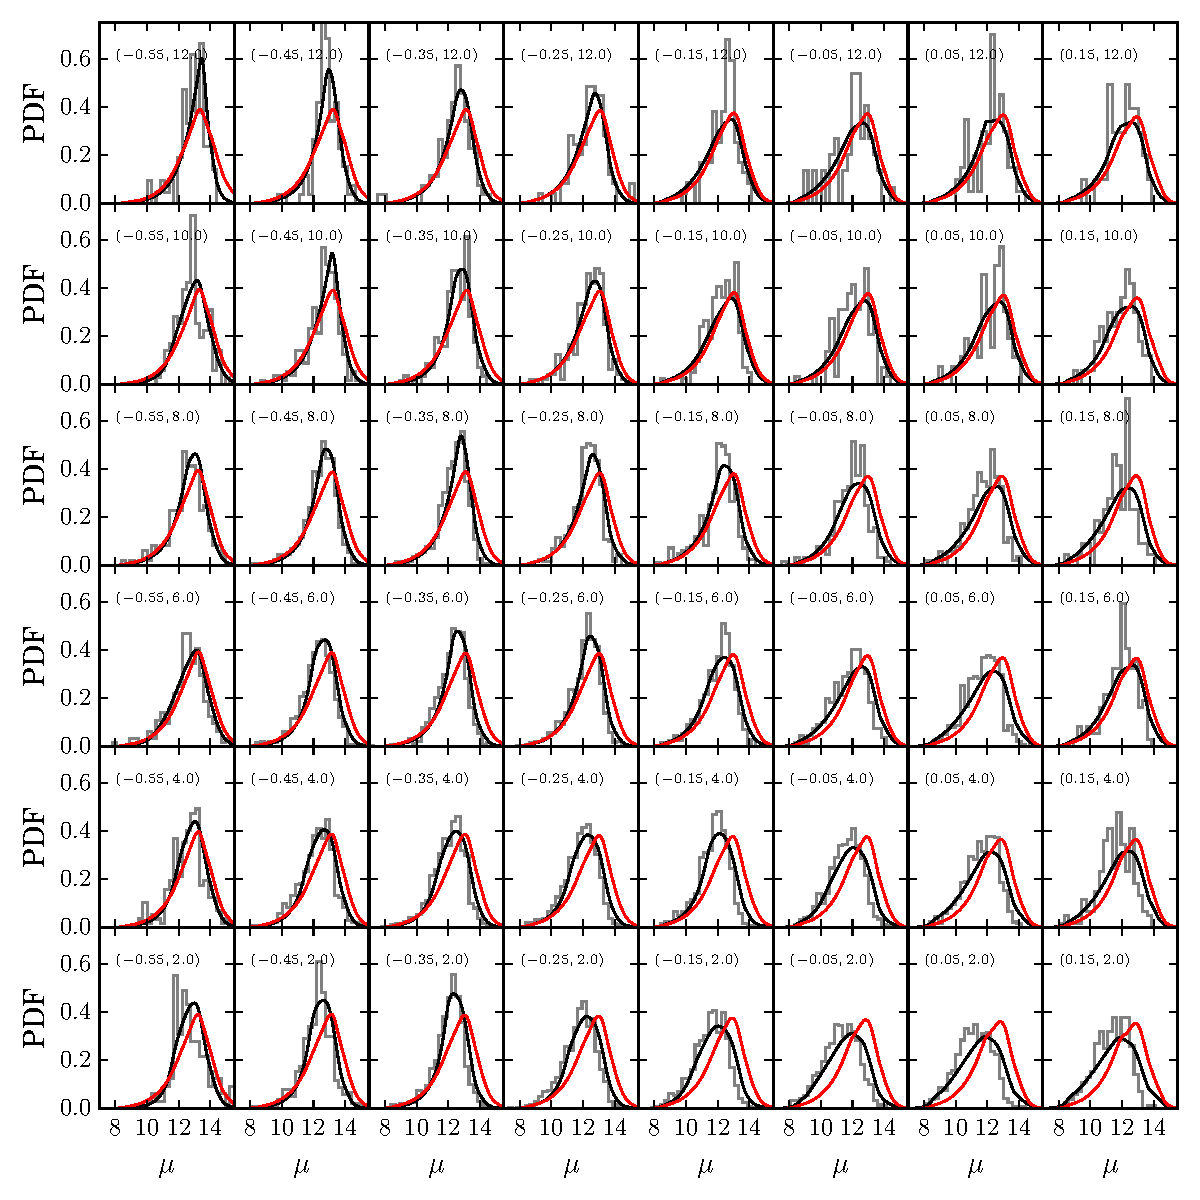
\includegraphics[width=\textwidth]{low_fitcomparison.pdf}
   \caption[Comparison between the APOGEE DR12 data and best-fit density models for the low \afe{} mono-age, mono-\feh{} populations]{ Comparison between the best fit models and the APOGEE data for mono-age, mono-\feh{} populations in the low \afe{} sub-sample. The grey histogram shows the distance modulus distribution of the APOGEE data for the mono-age, mono-\feh{} bin indicated by the (\feh{} [dex], age [Gyr]) coordinate given in each panel, where each panel shows a different mono-age, mono-\feh{} bin. The coloured curves show the distance modulus distribution found when the best fit broken exponential (black) and single exponential (red) density model is run through the effective selection function. It is clear that the broken exponential density model provides a qualitatively better fit to the data in all cases.}
     \label{fig:low_fitcomp}
 \end{figure*}

 \begin{figure*}
      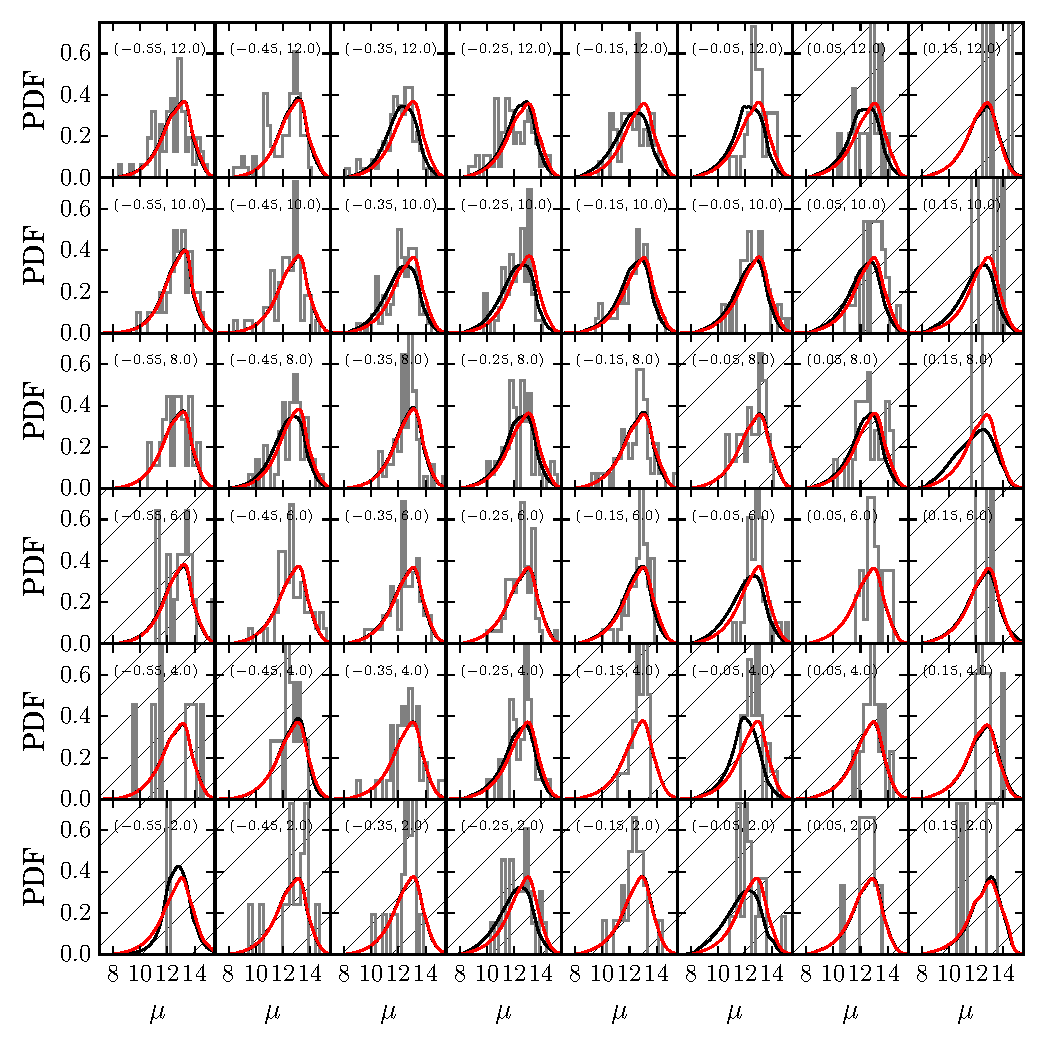
\includegraphics[width=\textwidth]{high_fitcomparison.pdf}
   \caption[Comparison between the APOGEE DR12 data and best-fit density models for the high \afe{} mono-age, mono-\feh{} populations]{Comparison between the best fit models and the APOGEE data for mono-age, mono-\feh{} populations in the high \afe{} sub-sample. Each panel again shows a different mono-age, mono-\feh{} bin. The grey histogram shows the distance modulus distribution of the APOGEE data for the mono-age, mono-\feh{} bin indicated by the (\feh{} [dex], age [Gyr]) coordinate given in each panel. The coloured curves show the distance modulus distribution found when the best fit broken exponential (black) and single exponential (red) density model is run through the effective selection function. In many cases the red and black curves are indistinguishable (only red is seen), or very similar. In cases where the black and red curves are different, the red provides a qualitatively better fit. Bins with less than 30 stars (which I disregard for the majority of the analysis and discussion) are hatched out. }
     \label{fig:high_fitcomp}
 \end{figure*}

 \section{The effect of uncertainties on trends with age}
 \label{sec:ageerror}


In order to demonstrate and characterise the effect that the age errors have on the interpretation of the trends between structural parameters and age, I use a mock data set with an input trend of $h_Z$ with age which increased monotonically with age from 0.2 to 1.2 kpc. Ages are assigned to each $h_Z$ population, sampling uniformly in bins of width 2 Gyr, to which I then added a random gaussian error of $40\%$, replicating the shifting of stars with different $h_Z$ into each age bin. In each bin, I sample a single exponential (a broken exponential with $R_\mathrm{peak}=0$) with scale length 8 kpc. This higher scale length is required to make the test computationally efficient, to produce realistic numbers of stars when selecting stars in APOGEE fields and does not impact on the results of this test. We assume no error on the stellar positions, in order to isolate the effect of the age errors. 

 \begin{figure}
      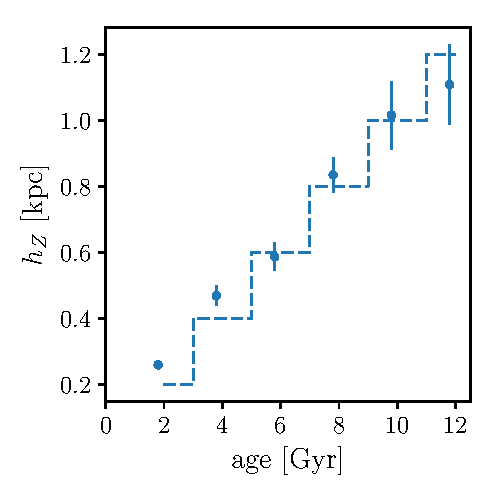
\includegraphics[width=0.5\columnwidth]{montecarlo_hz.pdf}
   \caption[Scale height vs. age for a Monte Carlo mock data set, intended to simulate the effect of age uncertainties on the trends recovered by the density fitting methodology]{The resulting age-$h_Z$ trend from the Monte Carlo sampling of a set of mock density distributions. The input  density models had $h_Z$ increasing monotonically with age (in bins of $\Delta\mathrm{age}= 2$ Gyr) from 0.2 to 1.2 kpc (shown by the \emph{blue} dashed line). After sampling of the density distribution, random errors of $40\%$ were applied to the mock ages, and the structural parameters were measured using the exact density fitting method applied to the APOGEE data. The method is able to approximately recover the general shape of the input age-$h_Z$ relation, showing a clear trend with age. The age errors increase the error bar sizes significantly where mixing does occur, but the results are consistent with the input in most cases.}
     \label{fig:montecarlo_hz}
 \end{figure}

While this test is a somewhat simplistic representation of the underlying processes, it serves as a good example of the effect of the age uncertainties which are expected in the present data. One example of its simplicity is the assignment of a single $h_Z$ to relatively wide bins in age. It seems logical to assume that if there is an age-$h_Z$ relation, then the change in $h_Z$ should be somewhat continuous with age. This test assigns the same $h_Z$ to stars at bin edges (which should have $h_Z$ close to that of the bin-edge stars in the neighbouring bin). This may artificially increase the amount of blurring of the age-$h_Z$ trend. I also simplify the test by assuming that the only changing parameter is the scale height. Realistic structural parameters would change the relative number of stars within each bin observed by APOGEE (and considered in our test), and may change the level of contamination between bins. However, this simple approximation represents a `worst case' scenario, where the mixing between bins is maximal.

I restrict the mock data to the APOGEE fields, simplifying the selection function to a distance cut (assuming the selection fraction is 1 out to a distance which corresponds to $M_\mathrm{H}= -1.5$, assuming no extinction).  I apply the method described in Section \ref{sec:methoda} to the mock data, fitting a broken exponential profile, and using the best fit solution to initiate an MCMC sampling of the posterior probability distribution. As in the main body of the paper, the reported parameter values reflect the median and $\sigma$ of one dimensional projections of the MCMC chain. The resulting age-$h_Z$ relation is shown in Figure \ref{fig:montecarlo_hz}.  A clear trend is recovered between age and $h_Z$. The trend is still recovered at high age, regardless of the high level of mixing between bins, which increases the size of the error bars. The higher-scale height components are recovered by the analysis, but results are scattered around the input values, with large error bars. This serves to show that even in the face of large age uncertainties causing mixing between the adopted bins, this method is still able to recover the underlying trends of parameters with age.

